\section{Extreme Value Theory. }
\begin{frame}[plain]
        \vfill
      \centering
      \begin{beamercolorbox}[sep=8pt,center,shadow=true,rounded=true]{title}
        \usebeamerfont{title}\insertsectionhead\par%
        \color{oxfordblue}\noindent\rule{10cm}{1pt} \\
        \begin{itemize}
        \item Normal Choices are POT or Block Maxima, but these strategies require
              large amounts of data to converge~\cite{taleb2019much}.
        \item \texttt{skextreme}~\cite{skextremes} is an python package that implements these
              standard strategies.
        \item Taleb does present some solutions~\cite{taleb2019statistical}.
        \item As physical processes with understood causes, TCs
              and their storm surges are \texttt{grey not black swans}.
        \item Need to know bias between hourly to daily output.
        \end{itemize}
      \end{beamercolorbox}
      \vfill
\end{frame}


\begin{frame}{Initial Block Maxima EVT }
\begin{itemize}
    \item The Block Maxima method with the ORCA12
    \texttt{control-1950} seemed easier to initially implement.
    \item Whether POT or BM converges faster depends
          on the underlying distribution~\cite{bucher2018horse}.
    \item The input is the 101 yearly maxima for each of the points along the coast,
         relative to the deviation from the long term mean.
    \item I initially use two different BM modules in \texttt{skextreme}.
    \end{itemize}
    \end{frame}
    \begin{frame}{GEV Equations }
    \begin{itemize}
\item
\(
\operatorname{GEV}(\mu, \sigma, \xi):
\)
\(
\text{ location, } \mu \in \mathbb{R}
\text{; scale, } \sigma>0
\text{; shape, } \xi \in \mathbb{R}.
\)
\begin{eqnarray}
\operatorname{GEV}(x; \mu, \sigma, \xi)=&
\frac{1}{\sigma} \chi(x)^{\xi+1} e^{-\chi(x)};\\
\chi(x)=&\left\{\begin{array}{ll}
\left(1+\xi\left(\frac{x-\mu}{\sigma}\right)\right)^{-1 / \xi} & \text { if } \xi \neq 0 \\
e^{-(x-\mu) / \sigma} & \text { if } \xi=0
\end{array}\right.
\end{eqnarray}
\item The Gumbel distribution is a special case ($\xi=0$)

\begin{equation} \operatorname{GUM}(x ; \mu, \sigma)=e^{-\frac{x-\mu}{\sigma}-e^{-(x-\mu) / \sigma}}
\end{equation}
\end{itemize}
\end{frame}


\begin{frame}{Leiblein New Orleans}
\vspace{-20pt}
    %\centering
 \begin{minipage}{1.0\textwidth}
\begin{figure}[htb!]
    \centering
    \includegraphics[width=1\linewidth]{../surge/plots/Lieblein_modelNO.pdf}
    \vspace{-15pt}
   \caption{Interesting transition - does this represent hurricanes? }
    \label{fig:}
\end{figure}
\end{minipage}
\end{frame}


\begin{frame}{Leiblein Miami}
\vspace{-20pt}
    %\centering
 \begin{minipage}{1.0\textwidth}
\begin{figure}[htb!]
    \centering
    \includegraphics[width=1\linewidth]{../surge/plots/Lieblein_modelMM.pdf}
    \vspace{-15pt}
   \caption{Fits Line well. }
    \label{fig:}
\end{figure}
\end{minipage}
\end{frame}


\begin{frame}{Leiblein Along Coast}
\vspace{-20pt}
    %\centering
 \begin{minipage}{1.0\textwidth}
\begin{figure}[htb!]
    \centering
    \includegraphics[width=1\linewidth]{../surge/plots/skextreme_first_tactic.pdf}
    \vspace{-15pt}
   \caption{. }
    \label{fig:}
\end{figure}
\end{minipage}
\end{frame}


\begin{frame}{GEV New Orleans}
\vspace{-20pt}
    %\centering
 \begin{minipage}{1.0\textwidth}
\begin{figure}[htb!]
    \centering
    \includegraphics[width=1\linewidth]{../surge/plots/GEV_modelNO.pdf}
    \vspace{-15pt}
   \caption{. }
    \label{fig:}
\end{figure}
\end{minipage}
\end{frame}

\begin{frame}{GEV Miami}
\vspace{-20pt}
    %\centering
 \begin{minipage}{1.0\textwidth}
\begin{figure}[htb!]
    \centering
    \includegraphics[width=1\linewidth]{../surge/plots/GEV_modelMM.pdf}
    \vspace{-15pt}
   \caption{. }
    \label{fig:}
\end{figure}
\end{minipage}
\end{frame}

\begin{frame}{GEV Models Along Coast}
\vspace{-20pt}
    %\centering
 \begin{minipage}{1.0\textwidth}
\begin{figure}[htb!]
    \centering
    \includegraphics[width=1\linewidth]{../surge/plots/skextreme_second_tactic.pdf}
    \vspace{-15pt}
   \caption{. }
    \label{fig:}
\end{figure}
\end{minipage}
\end{frame}


\begin{frame}{There is a physical maximum given the climatology.}

\vspace{-30pt}
\begin{figure}[htb!]
    \centering
    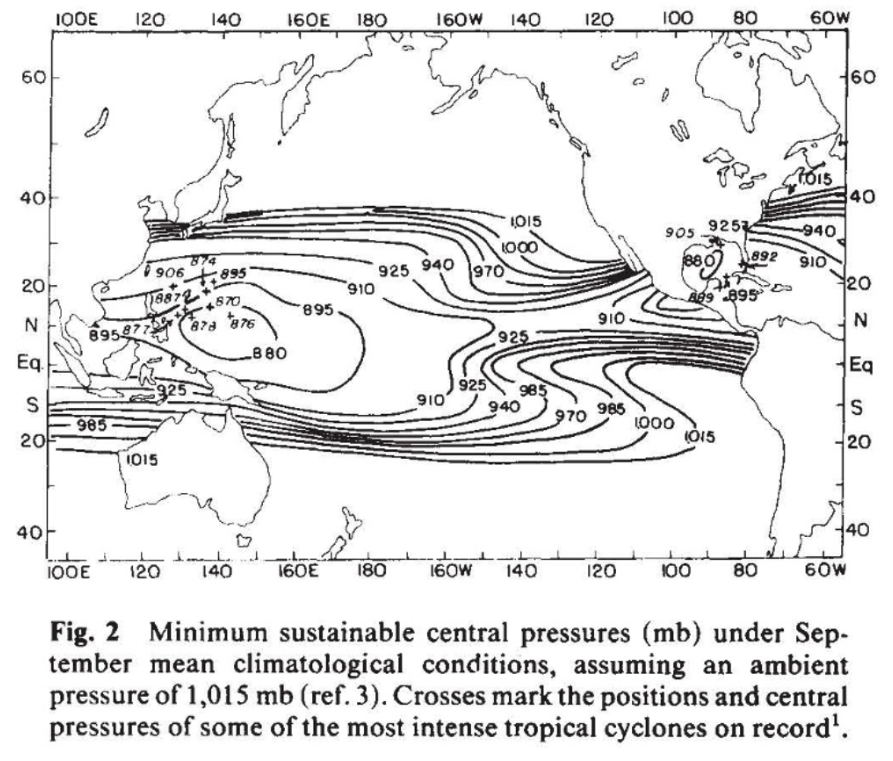
\includegraphics[width=0.8\linewidth]{images/hurricane-Emanuel-upper-bound.png}
    \vspace{-15pt}
   \caption{\cite{emanuel1987dependence} }
    \label{fig:}
\end{figure}
\end{frame}

\begin{frame}{So could we do something more intelligent?~\cite{taleb2019statistical}}
\vspace{-20pt}
    %\centering
 \begin{minipage}{1.0\textwidth}
\begin{figure}[htb!]
    \centering
    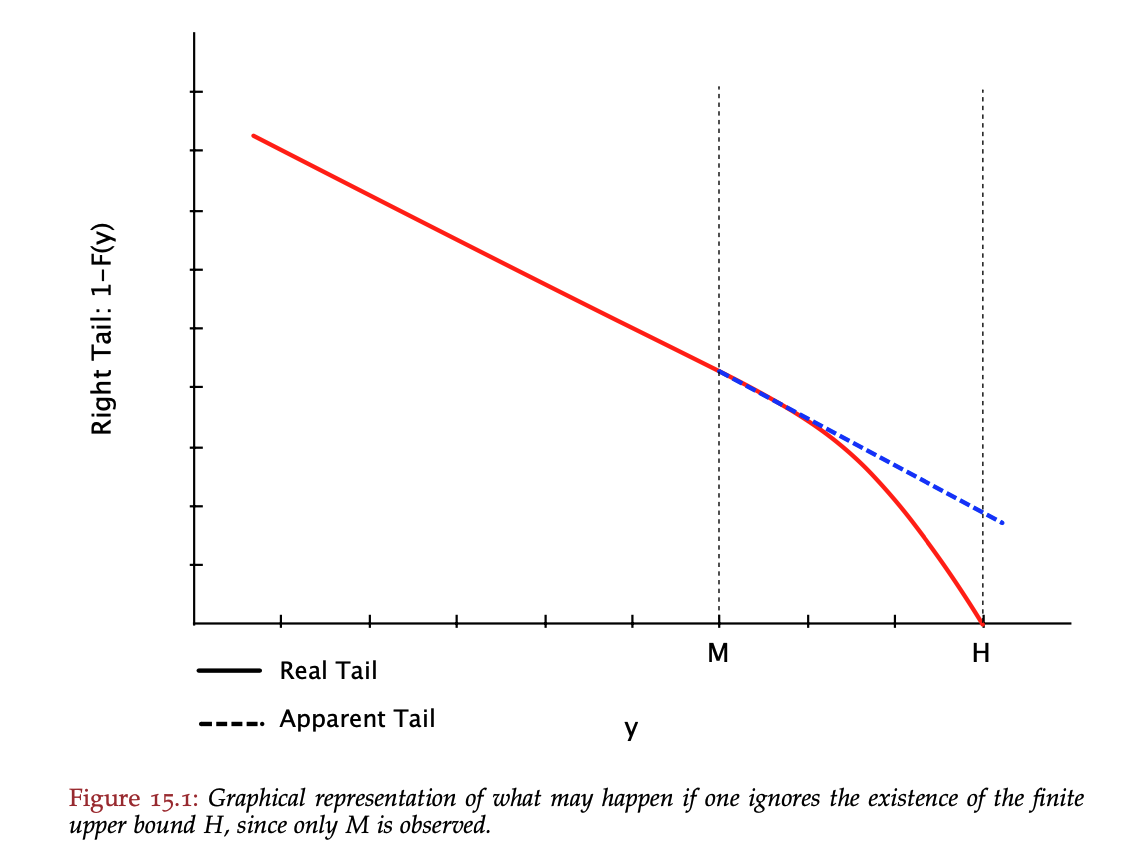
\includegraphics[width=1\linewidth]{images/nnt-upper-bound.png}
    \vspace{-15pt}

   %\caption{. }
    % \label{fig:}
\end{figure}
\end{minipage}
\end{frame}
